\documentclass[a4paper]{scrbook}
\usepackage[T1]{fontenc}	% Fontencoding for pdf searches
\usepackage{textcomp}		% EUR symbol for OT and T1
\usepackage[osf,sc]{mathpazo}	% Palatinofont
\usepackage{ellipsis}		% better spaces for ellipses (…)
\usepackage{microtype}		% Typographic finetuning
\usepackage{fixltx2e}		% LaTeX fixes

\usepackage[euler]{textgreek}
\usepackage[utf8]{inputenc}	% utf8 input
\usepackage{graphicx,framed}	% pictures, frames
\usepackage{makeidx}		% Index
%\usepackage{fancyhdr}
\usepackage{listings}		% source listings, e.g. for shell commands

\usepackage{flafter}		% floating objects
\usepackage{placeins}		% \FloatBarrier command, http://www.tex.ac.uk/cgi-bin/texfaq2html?label=floats
\usepackage{color}		% colors
\usepackage{tikz}		% draw stuff
\usepackage{enumerate}		% more enumerations
\usepackage{longtable}		% multipage tables
\usepackage{booktabs}		% better tables: http://www.ctan.org/tex-archive/macros/latex/contrib/booktabs/

\usepackage[nottoc]{tocbibind}	% Index + Bibliographie -> toc

%\setcounter{tocdepth}{3} % Depth for tocs; default = 2

%PDF stuff
\usepackage[unicode,linktocpage,
colorlinks,
bookmarks,
bookmarksopen,
pdfpagelabels=true]{hyperref}

% pdf-spezifisches, no line breaks!
\usepackage{xcolor}
\hypersetup{
	pdftitle = {Cockatrice Usermanual},
	pdfsubject = {Cockatrice, Servatrice, Manual},
	pdfauthor = {},
	pdfkeywords = {Cockatrice, Servatrice, Magic},
	%linkcolor=blue!30!black,
	%citecolor=green!30!black,
	%urlcolor=blue!25!green!25!black,
	linkcolor=black,
	citecolor=black,
	urlcolor=black,
	% Links nicht unterstreichen
	frenchlinks,
	% Links umbrechen
	breaklinks = true,
}

% better Text/Float-ratio
\setcounter{topnumber}{3}
\renewcommand\topfraction{1}
\setcounter{bottomnumber}{3}
\renewcommand\bottomfraction{1}
\setcounter{totalnumber}{9}
\renewcommand\textfraction{.01}
\renewcommand\floatpagefraction{1}

\makeindex
%opening
\title{Cockatrice}
\subtitle{Usermanual}

%\pagestyle{fancy}

\newcommand{\shellcmd}[1]{\texttt{\scriptsize #1}}

\begin{document}
\maketitle
\tableofcontents

\chapter{Preface}
This manual is basically a dump from the cockatrice.de dokuwiki. Cockatrice has some legal problems right now and the page is down.
This document tries to save the documentation about the software, beautify and extend it in the future.
Please contribute to the project, it is much too precious to be destroyed.

\chapter{Getting Started}
\section{Making A User Profile}
Not available anymore, site is down. 
If someone runs his own server where you can register a user profile, read his documentation.

\section{Downloading and Installing the Cockatrice Program}
Due to a legal dispute there are currently no official builds left, so currently you have to build your own binaries.

\subsection{Client compilation}
\subsubsection{Windows}
TODO, please contribute this section!

\subsubsection{Install latest experimental on Linux}
\begin{enumerate}
 \item You need to install the build tools and dependencies. This varies between the Linux distributions.
 \begin{description}
  \item[Ubuntu] \shellcmd{sudo apt-get install build-essential git libqt4-dev qtmobility-dev libprotobuf-dev protobuf-compiler cmake}
  \item[Fedora] \shellcmd{sudo yum groupinstall "Development Tools"\\
  yum install qt-devel qt-mobility-devel protobuf-devel protobuf-compiler cmake}
 \end{description}
 \item Download the sources from github via \\ \shellcmd{cd\\ git clone https://github.com/Daenyth/Cockatrice.git}
 \item To compile the sources, change into the newly created directory, create a build directory and invoke cmake:\\
 \shellcmd{cd Cockatrice \\
mkdir build \\
cd build \\
cmake ..\\
make\\
sudo make install
}\\
If you have some issues with pthread\_* add 'pthread' to the ``target\_link\_libraries'' entry in the \shellcmd{CMakeFiles.txt} in \shellcmd{Cockatrice/common}.

 \item Finish up the installation: Run \shellcmd{oracle} and download available cards, denn run \shellcmd{cockatrice}.
The default paths for decks, pics, cards and tokens are located in \\ \shellcmd{/home/<user>/.local/share/data/Cockatrice/Cockatrice}.
\end{enumerate}

\subsubsection{MacOS X}
TODO, please contribute this section! See Linux section, then use the \shellcmd{prepareMacRelease.sh} script from Cockatrice.

\subsection{Server compilation}
You don't need your own server if you plan to play only. But as Cockatrice is open source you are free to run your own.
The compilation works like already written above, but instead of invoking \shellcmd{cmake ..}, you have to do it like this:
\begin{itemize}
 \item If you want to build the server, use:\\ \shellcmd{cmake -DWITH\_SERVER=1 ..}
 \item If you want to build the server, but not the client, use:\\ \shellcmd{cmake -DWITH\_SERVER=1 -DWITHOUT\_CLIENT=1 ..}
\end{itemize}

\section{Downloading Card Database Using the Oracle}
If you are installing Cockatrice for the first time, changing what sets are in your database or even adding the newest set to your database, this tutorial will show you how to do it properly.

The Oracle will automatically run after the initial setup of Cockatrice. If you would like to re-install your database or add new sets you can find it (for Windows) by clicking the start menu, going to all programs, selecting the Cockatrice folder, and in there you will find the Oracle tool.
\begin{itemize}
 \item When the Oracle importer opens, click on “File” in the top left corner and select “Download sets information…”
 \begin{center}
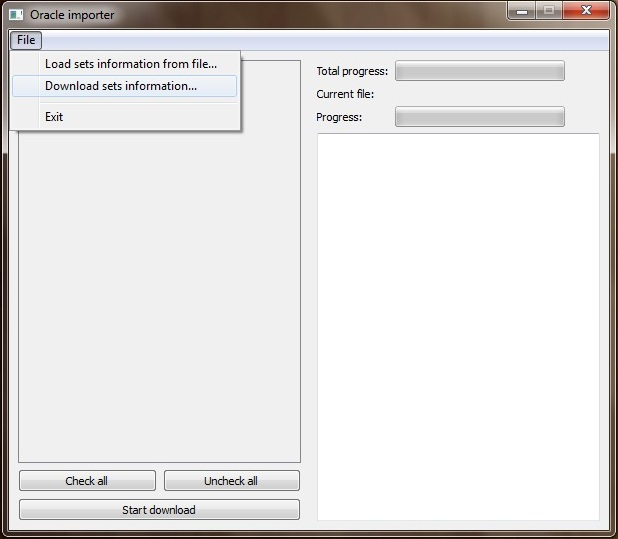
\includegraphics[scale=0.8]{pics/fetch554a}
 \end{center}
 \item This will bring up a box where you can input the URL of a card database. The default address is \url{http://www.cockatrice.de/files/sets.xml} this was an XML file found on the Cockatrice website that has the current set listings for Magic the Gathering. As the page is down, you have to import the file which is distributed with the Cockatrice sources.
 This can also be done from the file menu.
 \item Select “OK” to load the set listings.
 \item A list of all current sets will be brought up. A default selection of sets will automatically be checked. From here you can check or uncheck all sets, or you may only download specific sets that you wish to play with.
  \begin{center}
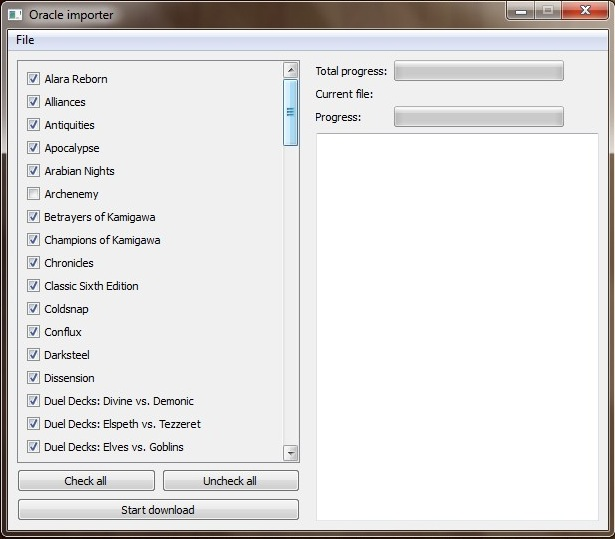
\includegraphics[scale=0.8]{pics/fetchfc3d}
 \end{center}
NOTE: If you are playing against someone who is using a card that is not in your database, you will not see a card image or oracle text for that card. Some players like to download all sets to avoid this issue, but other players who only play specific formats (Like \textsc{T2}, \textsc{Standard}, or \textsc{Extended}) wish to keep their database small with only cards they will be using.
 \item After you select which sets you wish to download, select “Start download” at the bottom of the Oracle to download the selected sets information.
 \item After download is complete, close the Oracle and run Cockatrice.
 \item We are now ready to sort our set information in our deck editor.
\end{itemize}

\section{Editing Set Order and Preference of Card Art}
Many cards have been re-printed in different sets, and in return have different versions of artwork (like the card “Cancel” which can be found in many sets, but has different artwork for each, e.g. \textsc{Zendikar} versus \textsc{M11}:
\begin{center}
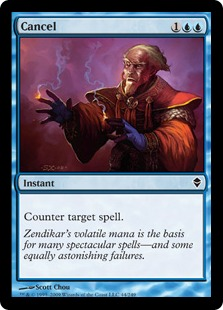
\includegraphics{pics/fetchc18b}
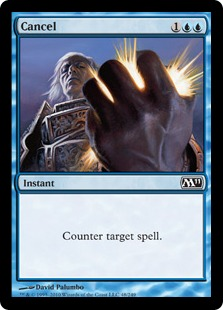
\includegraphics{pics/fetche1f4}
\end{center}

Some players like to have the most current artwork displayed on their cards, while other players have a favorite set they wish to display instead.

\begin{itemize}
 \item Run Cockatrice and select “Deck editor” from the top right Cockatrice menu. This will bring up the Deck Editor along with a list of all cards that are currently in your database which you downloaded using the Oracle Tool.
 \item To change what version of the cards will be shown, click on “Card database” on the top left of the Deck editor window, and select “Edit sets…”
  \begin{center}
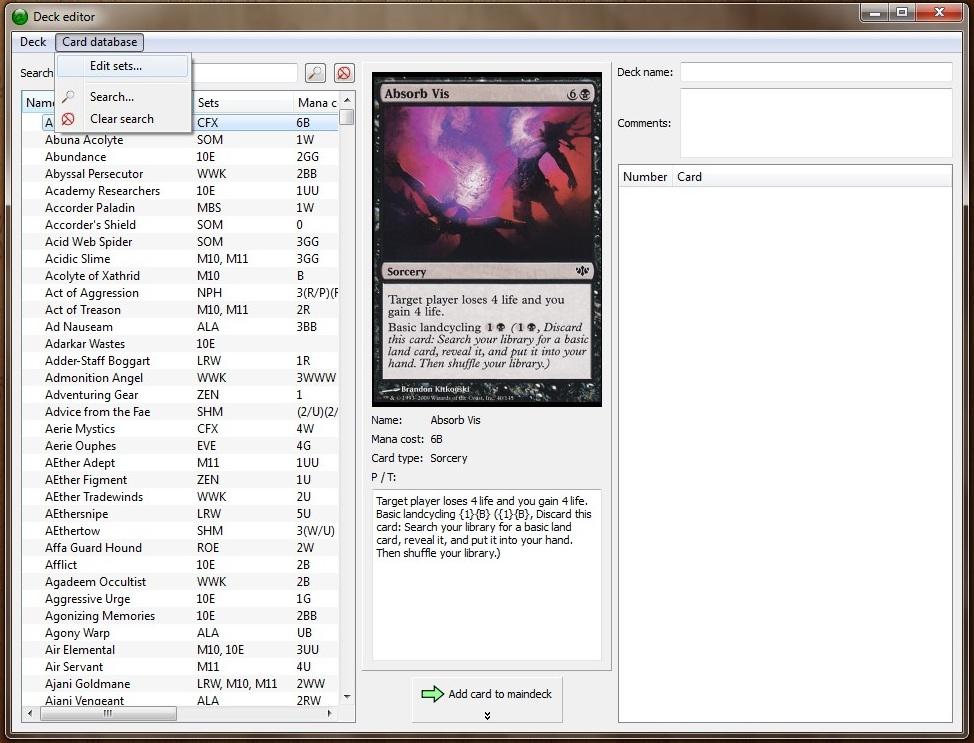
\includegraphics[scale=0.55]{pics/fetchf924}
 \end{center}
 \item This will bring up a new window that has a list of all sets you currently have downloaded to your database. To change the order of the sets, simply drag and drop them into place.
 This will determine which artwork is shown for your cards. If a card is found in multiple sets, whichever set is closest to the top of this list will be the art displayed.
 Example: If \textsc{M11} is above \textsc{Zendikar}, The M11 version of the card “Cancel” will be displayed in your Deck editor and Cockatrice games.
\end{itemize}
NOTE: Your opponent will NOT see what artwork you have selected for each of your cards. They will only see what they have selected for their own. 

\section{The Deck Editor / Making a Deck}
The Cockatrice Deck Editor is a tool you can use to make decks to play online.
The cards shown in the Deck Editor are from a database that you downloaded with the Oracle Tool. If you are missing cards or a new set has come out, you must re-run the Oracle and download set information.
\begin{center}
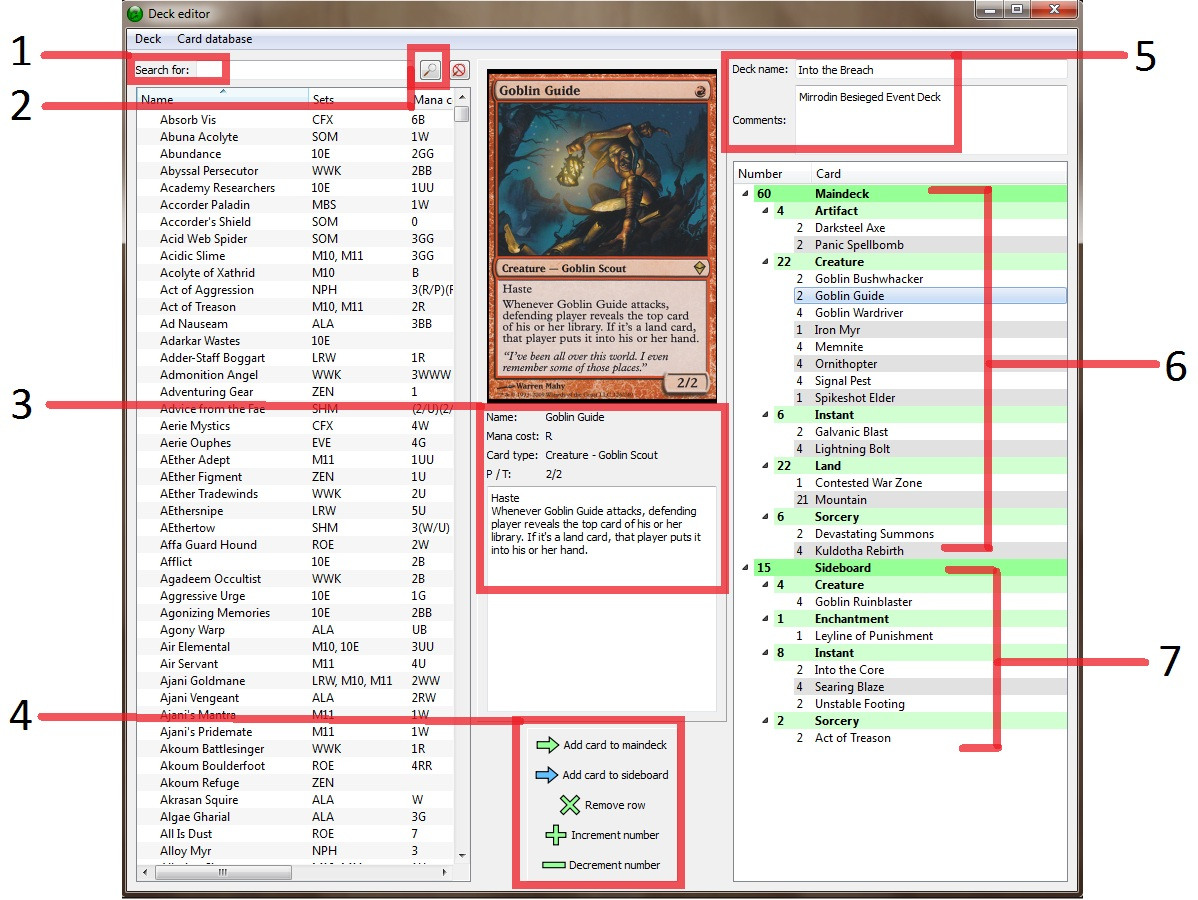
\includegraphics[scale=0.55]{pics/fetch52e0}
\end{center}

\begin{description}
 \item[1. Search Bar] The search bar lets you type in the name of a card and the editor will only show cards that start with whatever you typed in. Example: Typing in ‘B’ will show all cards that start with the letter ‘B’ and typing in ‘Dark’ will show you all cards that start with ‘Dark’ and so on. If you were looking for the card “Sun Titan”, you would not type in ‘Titan’ you would have to type in ‘Sun’ first. Typing in ‘Titan’ will only show you any cards that start with ‘Titan’.
 \item[2. Card Search/Filter] The Card search button will bring up a new window that helps you filter out cards more specifically. A variety of check boxes will help find what you need. Card name lets you filter out only cards that have a cretin word in them. Card text can help you find key words like “Haste” or “Infect”. If you were to uncheck all boxes except for “Instant” along with “Artifact” and “U”, the Deck editor will only show you all Blue Instant and Artifact cards.
\begin{center}
\begin{tabular}{ll}
\toprule Letter & Card Type \\ \midrule
U  & Blue \\ 
W  & White \\ 
X  & Colorless \\ 
G  & Green \\ 
R  & Red\\ 
B  & Black \\ \bottomrule
\end{tabular}
\end{center}
 \item[3. Card Data] This section shows the Oracle text for the card that you currently have selected. It will show you up-to-date information on the card such as the Name, Mana cost, Card type, Power/Toughness, and any abilities the card has. It will not show you flavor text.
 \item[4. Adding/Removing Card Buttons]
The buttons in the bottom middle will add or remove cards from your Deck List, as well as ad a card specifically to your Sideboard. Having a card selected on the left column and hitting the Enter key will also add it to your deck list.
 \item[5. Deck Name/Comments]
The area in the top right lets you name your deck as well as give any comments or descriptions such as how to play the deck, where the deck came from, or explain a theme. Putting something in the “Deck Name” space will NOT be what the file name of the file for your deck. That is spate in the “save” selection under the “Deck” menu found at the top left of the Deck Editor window.
 \item[6. Main Deck List]
This area will show you what cards you currently have added to your deck list. It is sorted by card type and also shows you how many of each card and card type you have added, as well as keeps track of how many total cards you have added to your main deck list. This will not add any number of cards you have added to your Sideboard.
 \item[7. Sideboard List]
The bottom section of the deck list shows any cards you have added to your sideboard. Again these are split into card types and it will keep track of how many of each card you have as well as how many of each card type and total cards in sideboard. This section will not add any cards from the main deck. Once you have all of your cards added to your deck, you must save it as a file Cockatrice can read. Select “Deck” from the top left corner of the Deck Editor screen, and select “Save Deck” or “Save Deck As…” and it will bring up a new window where you can select where you would like to save your deck, as well as assign it a file name. Cockatrice decks are saved as .cod files.
\end{description}

\section{Loading a deck list from your clipboard}
If you find a deck online, or you have a deck list saved in a word document, it is easy to transfer it over into a Cockatrice deck file as long as it is in a simple deck list format.
The simple deck list format is a list where each line begins with a number, followed by a whitespace, followed by the cardname, e.g.
\begin{verbatim}
2 Doom Blade
13 Island
10 Swamp
4 Cancel
...
\end{verbatim}

Simply find the word document or deck list online that you wish to save as a deck, and select the text and copy it to your clipboard. Next, open the Deck Editor screen, and click on the Deck menu from the top left corner. Select “Load deck from clipboard…” and the deck editor will bring up a new window that has the deck list you had copied to your clipboard. Make sure the Deck list looks correct and hit “OK” in the bottom right corner of the window. The Deck editor will now add all the cards in the list to your main deck list.

\begin{center}
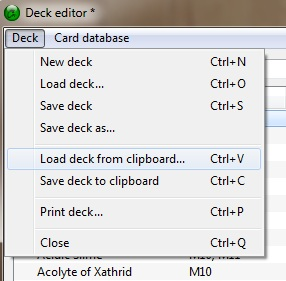
\includegraphics{pics/loaddeck_clip}
\end{center}

\begin{center}
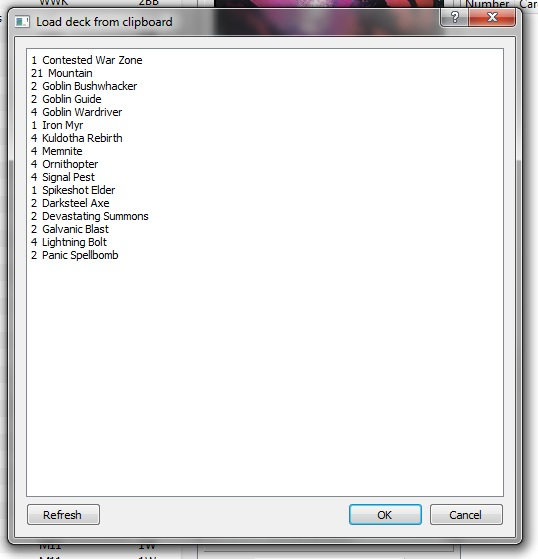
\includegraphics{pics/okdecklist}
\end{center}

NOTE: If you add a card to a deck list with this function that you do not have downloaded to your personal cockatrice database though the Oracle tool, the card will take a spot in your main deck list, and count toward the total number of cards, but it will show up as a blank image with no Oracle data or card information.

\section{Cockatrice Settings}
TODO

\section{Learning the Ropes / Starting a Solitaire Game}
The best way to get familiar with the way Cockatrice plays is to start a local game that you can play around in by yourself. You could also jump online and start slowly learning, and let other players help you.

To start a Solo Local game, in the main Cockatrice window, click on “Cockatrice” on the top left, and select “Start local game…”.

\begin{center}
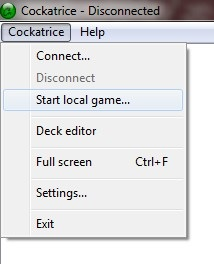
\includegraphics{pics/fetch2ab8}
\end{center}

This will bring up a small window that lets you select how many players will be in this local game you are creating. For right now, since we want to do a solo Solitaire game, select one player and hit “OK”.

\begin{center}
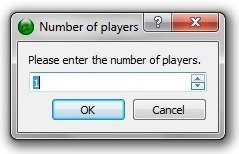
\includegraphics{pics/fetchf010}
\end{center}

\subsection{Loading a Deck / Using Sideboard}

This will now bring you to a screen where you load a deck to play with. On the top left part of this screen you will find a button that is labeled “Load Local Deck”. Click that button and it will bring up a window where you can find and select what deck you would like to play with.

\begin{center}
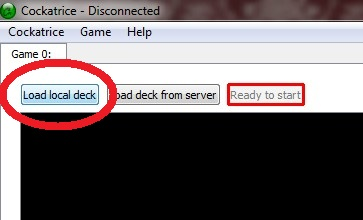
\includegraphics{pics/fetchf0d2}
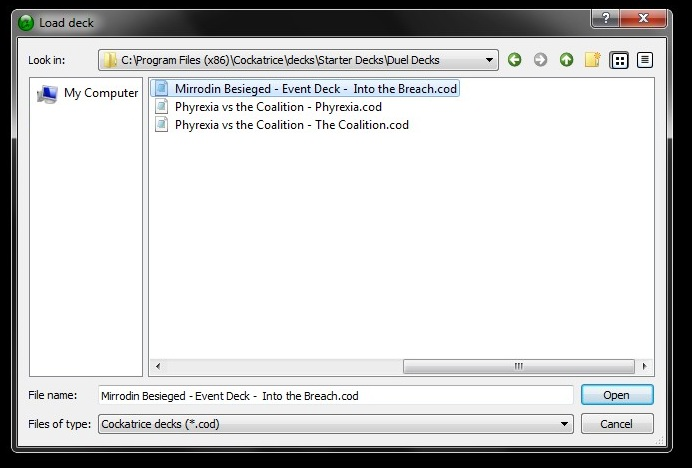
\includegraphics[scale=0.8]{pics/fetch55a7}
\end{center}
Select a deck or a .cod file and click “Open”.

\begin{center}
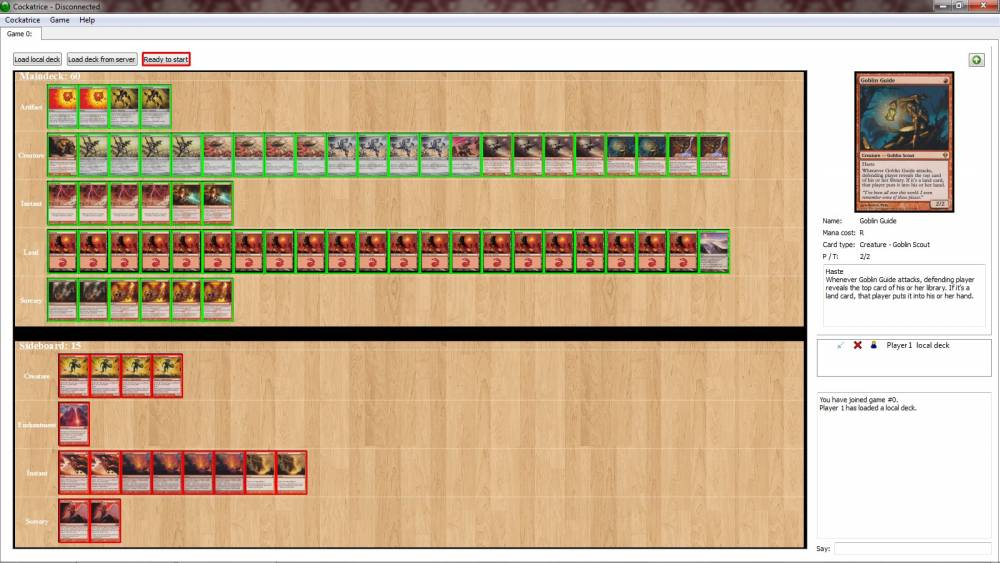
\includegraphics[scale=0.4]{pics/fetch9b89}
\end{center}

After the file has loaded you will see all of the cards in that deck laid out on the table. If you hover your mouse over a card, the card image and Oracle info will show on the right side of the screen. If you have a sideboard made for the deck there will be a second section on the table for this sideboard. This screen gives you the ability to double check your deck to make sure it is not only the correct deck you want to play with, but it lets you see that all card images have downloaded properly. If you have cards not showing up at all or they are just blank cards with names on them, you may not have that set downloaded with your Oracle tool. If you have a sideboard, you can drag and drop cards from your main deck to your sideboard or vice-versa. You can do this by clicking and dragging a card to or from your main deck or sideboard.

NOTE: Moving cards from your main deck to sideboard will NOT change how your deck file is saved, it will only change it temporary for the game you are playing or until you load a new deck.

When you are satisfied with your deck choice and/or sideboarding options, click on the red outlined “Ready to start” button found a the top of the screen.

\subsection{Finding Your Way Around}
The main game screenlooks like this
\begin{center}
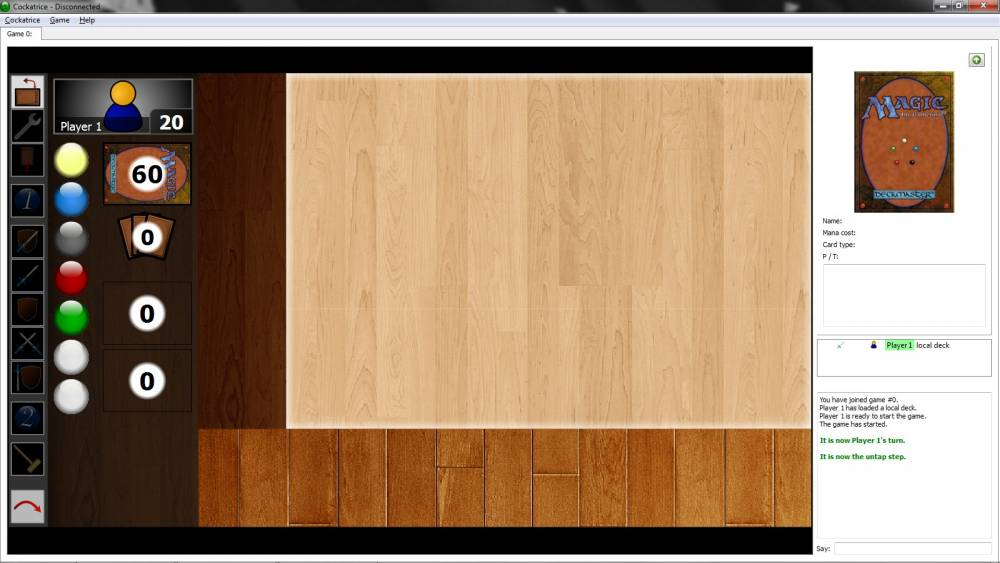
\includegraphics[scale=0.4]{pics/fetch7cf0}
\end{center}
(Please note your screen will look different due to background image options.)

\subsubsection{Main Table / Play area}
Split into four areas, this is where all the action will go down.
\begin{description}
 \item[The Stack] The area on the left side of the table where Instant and Sorcery cards will be played. This is for things that will only temporarily be put on the table, then into the graveyard. Multiple cards may be added to this area at the same time. Anything on this part of the table will be seen by all players.
 \item[Battlefield] This is the soul part of the game table. this is where creatures, enchantments, artifacts, and even plainswalkers will be placed. As cards are moved from your had to the table, they will be aligned to an invisible grid and moved around from there. Tap cards by double clicking them. Anything on this part of the table will be seen by all players.
 \item[Land] This space is for land cards, but any card may be placed here. Tap cards here by double clicking them. Anything on this part of the table will be seen by all players.
 \item[Hand] Every time you draw a card it will go here to your hand. You may also drag cards from the table back to your hand. Your opponents can not see what is in your hand.
\end{description}

\subsubsection{Player Info Section}
\begin{center}
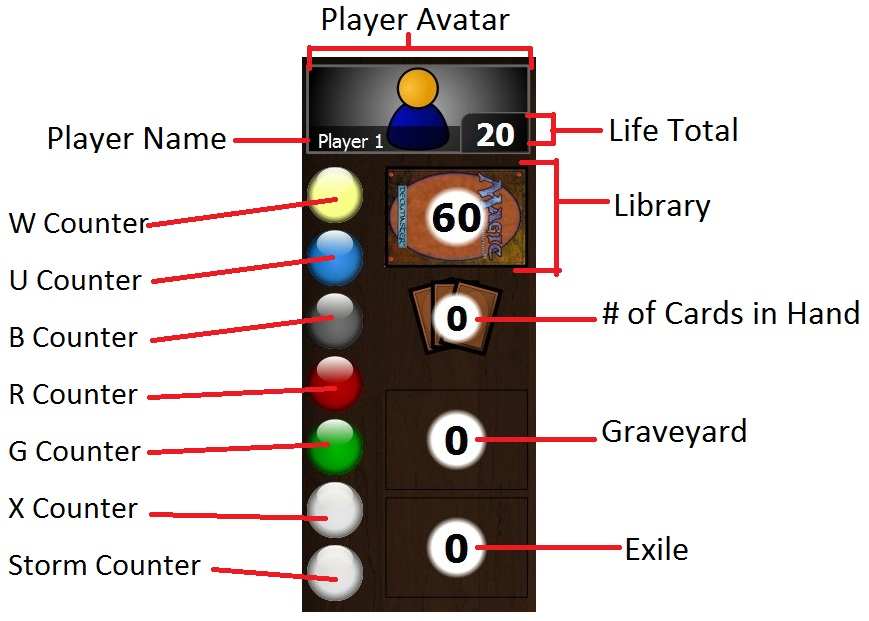
\includegraphics[scale=0.7]{pics/fetch0300}
\end{center}

\begin{description}
 \item[Player Avatar] This is a $156\times 60$ pixel JPG image that can be uploaded though the main Cockatrice website. All players in the game room can see this image. It serves nothing more than an online identity for you and other players.
 \item[Player Name] Your online name that you picked though the main Cockatrice website.
 \item[Life Total] Your in-game life. Using your mouse, if left-clicked will raise this number by one, and if right-clicked lowered by one. There are also keyboard shortcuts to change your life total.
 \item[Counters] These seven multicolored circles are used as counters. They can be seen by all players and can be changed by left or right clicking on them to add or subtract a number. Players use them for various digit counting but primarily used for adding and subtracting floating mana produced by card effects. The bottom two white counters can be used for other things like Poison.
 \item[Library] This is your deck of cards. The number in the middle reflects how many cards are left in your library. Double clicking the deck lets you draw a card and add it to your hand, you can also drag cards off the top into the battlefield or to your hand. Right-clicking the deck brings up a menu that allows other things to happen like reviling the top number of cards, shuffling, or moving cards directly into the graveyard.
 \item[Number of cards in hand] The number in the middle represents how many cards are currently in your hand. Other players can see this number but can not see the cards actually in your hand.
 \item[Graveyard] Cards can be dragged and dropped into your graveyard from play or vise-versa, the stack, your hand, or even your library. The number in the middle represents how many cards are currently in your graveyard. Any player may right-click on the graveyard and bring up a menu that shows what cards are in it.
 \item[Exile] Cards can be dragged and dropped into exile from play or vise-versa, the stack, your hand, or even your library. The number in the middle represents how many cards are currently in your exile. Any player may right-click on the exile and bring up a menu that shows what cards are in it.
\end{description}

\subsubsection{Turn Phases}
\begin{center}
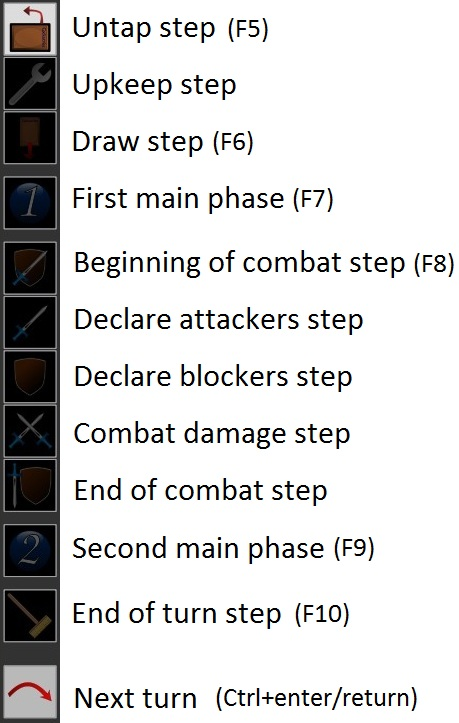
\includegraphics[scale=0.7]{pics/fetchfebd}
\end{center}
This bar located on the left most side of the screen represents the 11 steps in a players turn. To go from one phase to the next, you can click on the square of the phase you want to move to, or you can hit Ctrl+space to move down to the next. Some phases even have their own keyboard shortcut. Going from one phase to the next does not actually do anything to your or your cards, it is only a place marker for your opponents to see and keep up with what you are doing in your turn. For example, clicking to the “Draw Phase” will not automatically draw you a card. It is customary for a player to end their turn on the “End of turn step” and let their opponent hit the “next turn” button. This is a courtesy for other players if they wish to do something like use an instant at the end of your turn, or in response to something you did.

NOTE: Players sometimes use the term EOT which stands for “End Of Turn”. This is to let other players know they are doing something in response to the end of the current turn.

\subsubsection{Info/Chat Bar}
\begin{center}
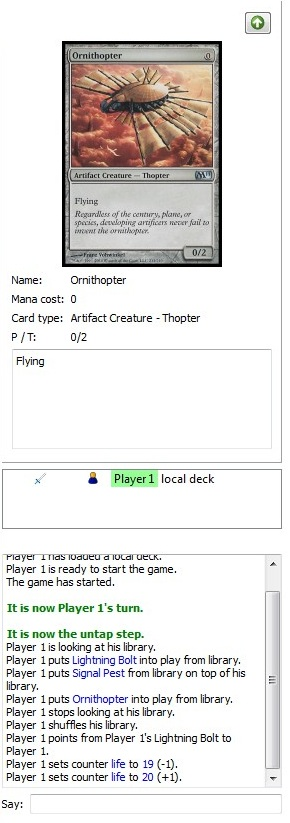
\includegraphics[scale=0.8]{pics/fetcha0de}
\end{center}
Split into three sections, the Info/Chat bar lets you see a close-up image of the card your mouse was last over, as well as gives you the card info for that card. At the bottom of this bar there is a chat log that helps keep track of events during the game as well as lets you communicate with other players. if a card is placed on the table, pointed at, or tapped it will get noted in the chat log as well as has a link to the card that you can hover over and see an image of at the top of the bar.

\subsection{Basic Functions}
\subsubsection{Rolling Dice}
At the beginning of a game players decide who is going first by rolling a 20 sided die. In Cockatrice we do this by pressing Ctrl-I and hitting enter. Hitting Ctrl-I brings up a die window and lets you select how many sides you want on your die. Default is 20, and pressing enter will “roll” the die. This action will show up in the cat log at on the bottom right of the screen. You can also find this in the “game” menu at the top of the window, selecting “player” and clicking on “roll die…”
\begin{center}
 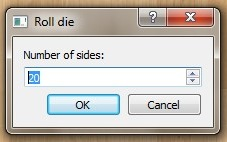
\includegraphics{pics/fetch7486}\\
 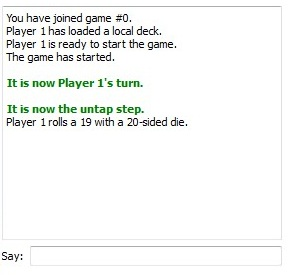
\includegraphics{pics/fetch3705}
\end{center}

\subsubsection{Draw Cards / Mulligan}
When a game starts and the first player has been selected, all players will draw seven cards. this can be done by pressing Ctrl-M. Seven cards will go from your library to your hand. Pressing Ctrl-M again will put the seven cards from your hand back into your library, shuffle your library and deal out six new cards to you. Each time you press Ctrl-M it will give you one less card until you get down to one card, then it will re-start at seven cards. This function can be found by clicking the “game” menu on the top of the window, selecting “player” then selecting “hand” and then “take Mulligan”. If you are playing a friendly game, press Ctrl-M as normal, but then press Ctrl-D to draw cards until you have a total of seven again.
\begin{center}
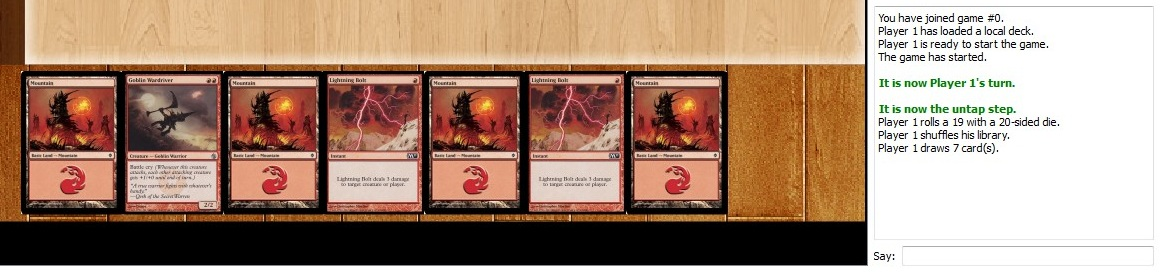
\includegraphics[scale=0.5]{pics/fetchfe20}
\end{center}


\subsubsection{Tapping}
Tapping cards is very basic. If a card is on the table under your control, you can double click it to tap it and then double click again to untap it. You can select multiple cards on the table by clicking and dragging your mouse, then tap or untap all of the selected cards at the same time. Other players can not tap or untap your cards. Pressing Ctrl-U will untap everything you control.

\begin{itemize}
 \item Untapped
 \begin{center}
  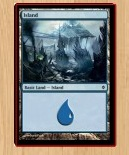
\includegraphics{pics/fetchb6fe}
 \end{center}

 \item Tapped
 \begin{center}
  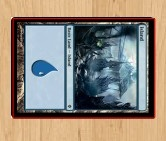
\includegraphics{pics/fetch867f}
 \end{center}
\end{itemize}

\subsubsection{Attaching Cards to Cards}
Sometimes an Enchantment -Aura or Equipment cards need to be attached to other cards that are already on the table. simply put the enchantment or equipment on the table. Right-click the card and select “attach” (this can also be done with Ctrl-A). A green arrow will appear, point and click on the card you wish to attach. You can also attach cards to other people's cards.
\begin{center}
 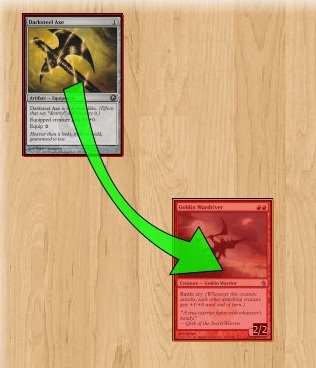
\includegraphics{pics/fetch100e}\\
 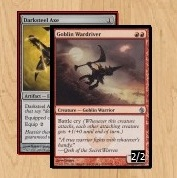
\includegraphics{pics/fetchb17a}
\end{center}


\subsubsection{Changing Power/Toughness}
Enchantments, Equipment, and other effects sometimes change a creatures power or toughness. This can be done by right-clicking the card, and selecting “power / toughness” then selecting which one you wish to do. Other players can not change your creatures power and toughness. This can also be done though a series of keyboard shortcuts seen below.

\begin{center}
\begin{tabular}{ll}
(Select card) Ctrl++ & Increase power \\
(Select card) Ctrl+- & Decrease power \\
(Select card) Alt++ & Increase toughness \\
(Select card) Alt+- & Decrease toughness \\
(Select card) Ctrl+Alt++ & Increase power and toughness \\
(Select card) Ctrl+Alt+- & Decrease power and toughness
\end{tabular}
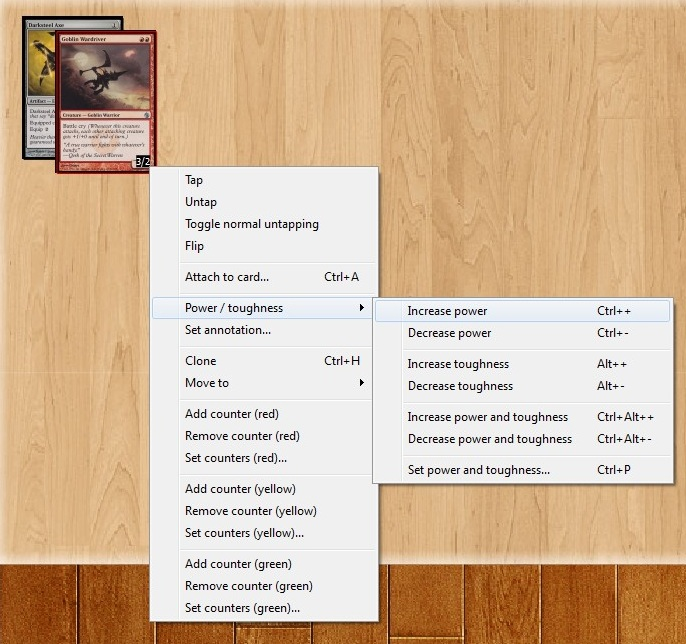
\includegraphics[scale=0.5]{pics/fetche3fc}\\
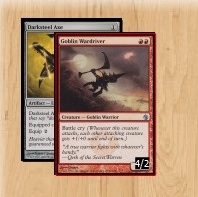
\includegraphics{pics/fetchd922}
\end{center}

\subsubsection{Adding Counters to Cards}
Sometimes Counters are needed to be placed on cards that the counters on the side of the screen are not able to track. Cockatrice offers three different counter color options, Red, Green, and Yellow. Although there is no set standard on what color stands for what, it is mostly player preference. Green could be used for +1/+1, red -1/-1, leaving yellow for charge and quest counters, this is not a set rule. Adding counters is as simple as right clicking on the card you wish to add counters too, and currently there is no keyboard shortcut for this process. Removing counters is the same process, right click and select remove. Other players can not add or remove counters to or from your cards.

\begin{center}
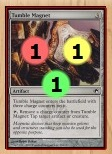
\includegraphics{pics/fetch5170}
\end{center}
(One of each counter)

\subsubsection{Pointing at Cards / Arrows}
Pointing at cars is needed for resolving spells, or declaring attackers and blockers. All you need to do is right-click over a card and drag an arrow over to what you are pointing at. Permanents, spells in the stack, and even a players life total can be pointed at. You can point at your opponents cards and life total, and they can point at yours. When your arrows are no loner needed, press Ctrl-R to remove them from the screen.

\begin{center}
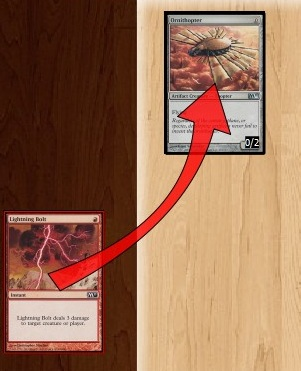
\includegraphics[scale=0.5]{pics/fetch98fd} \\
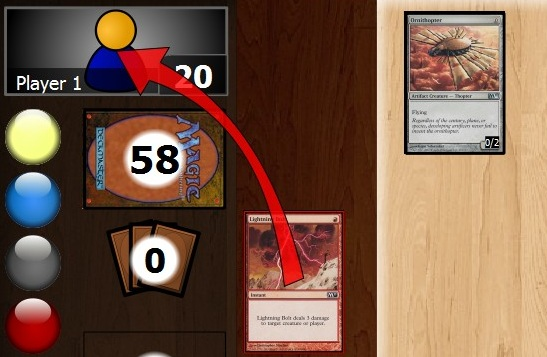
\includegraphics[scale=0.5]{pics/fetch74b2}
\end{center}

\subsubsection{Creating Tokens}
Creating tokens can sometimes be tedious, but is well worth the effort to keep a clean and organized game. Pressing Ctrl-T will bring up a small window to assist you in creating a token. Simply enter the name of the token you are creating, select its color, and give it a power and toughness (\#/\#). You can also bring up this token window by selecting “game” from the top menu, selecting “Player” then clicking on “Create Token…”. A copy of the Last token made can be done by pressing *Ctrl+G or right-clicking on a already made token (or any card on the table) and selecting “clone” or pressing Ctrl-H**. When a token or clone leaves play, it will be destroyed and vanish.

\begin{center}
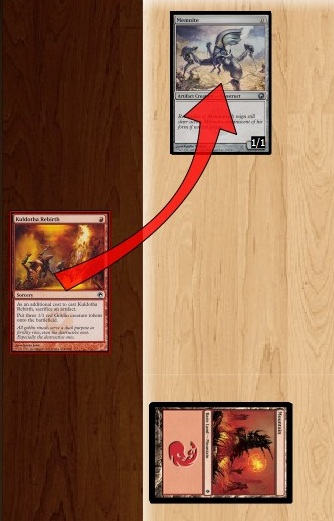
\includegraphics[scale=0.5]{pics/fetch2c36} \\
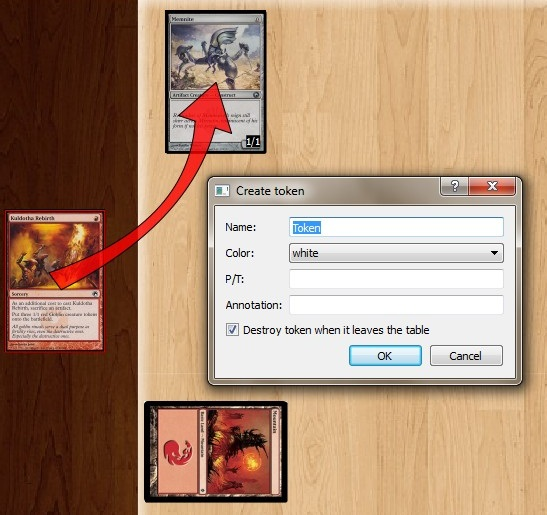
\includegraphics[scale=0.5]{pics/fetch9bff} \\
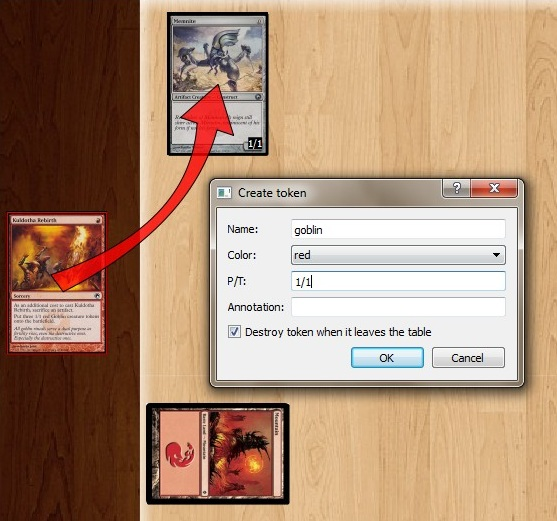
\includegraphics[scale=0.5]{pics/fetche6b2} \\
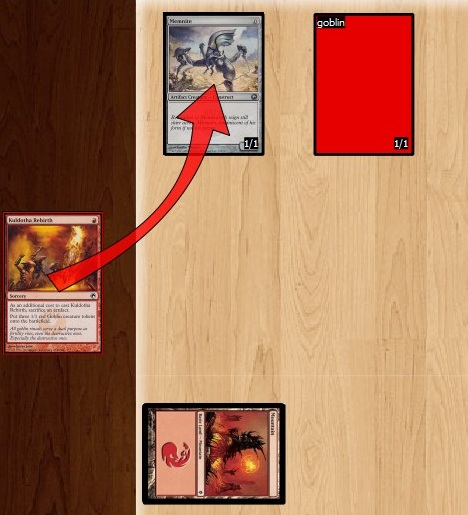
\includegraphics[scale=0.5]{pics/fetch84a2}
\end{center}

Make copies of your last token by pressing Ctrl-G.
\begin{center}
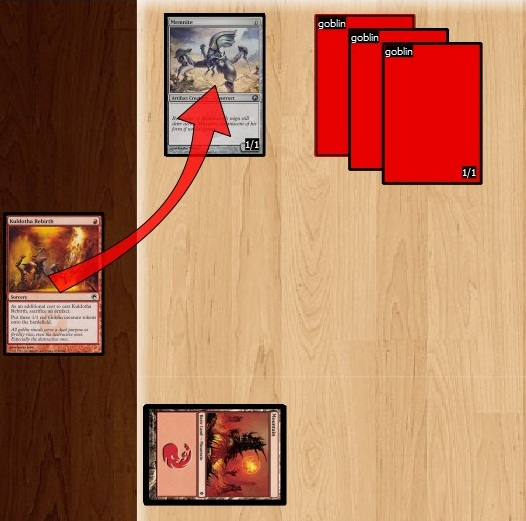
\includegraphics[scale=0.5]{pics/fetch6847}
\end{center}

\chapter{Playing Online}
 With Cockatrice you will most likely play Magic games over the Internet with real people all around the world. In order to help maintain a pleasant environment for users, please read the messages below:

\begin{itemize}
 \item User Code of Conduct\footnote{TODO, dead forum link} -- Must Read for all Users
 \item How to Report Abuse\footnote{TODO, dead forum link} -- It is recommended to read this as well 
\end{itemize}

\section{Connect to Server}
To connect to the Cockatrice server, launch the Cockatrice program, go to the “Cockatrice” menu at the top left, and select “Connect”. A window will appear (see image below).
\begin{center}
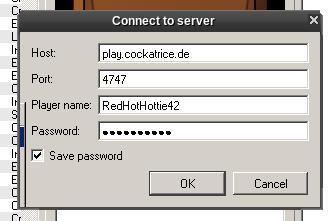
\includegraphics[scale=0.5]{pics/fetch23f3}
\end{center}
If you have registered with Cockatrice, then enter your Username in the “Player Name” field and your password in the “Password” field then click “OK”. You may check the “Remember Password” box if you wish. If you do, then the next time “Connect” is selected from the “Cockatrice” menu, the window that appears will already have your Username and Password already filled. Please take this into consideration if you share a computer with other people, seeing that you are responsible for anything that happens on the server with your username (As noted here). If you did not register with Cockatrice, then simply fill in the Username with whatever you like and click “OK”. If you would like to become a registered user, read the instructions from the server's website.

Once you are connected to the server, more tabs will appear at the top of the screen next to the “Deck” tab that you are already on.

\section{All About Games}
This page is about creating, joining, watching, and searching for games on the Cockatrice Server. In order to participate in any games, you have to be connected to the server. The games on the server are where all of the action take place. There will be many games happening on the server at the same time. Basically, first a game is created by a player (it could be you). Then other players join the game until the number of players reaches the number set by that game's creator. When the game has no players participating in it, the game disappears.
Creating a Game

To Create a game, go to the “MTG room” tab. Click on the “Create” button below the Games list. A window will appear (see below).
\begin{center}
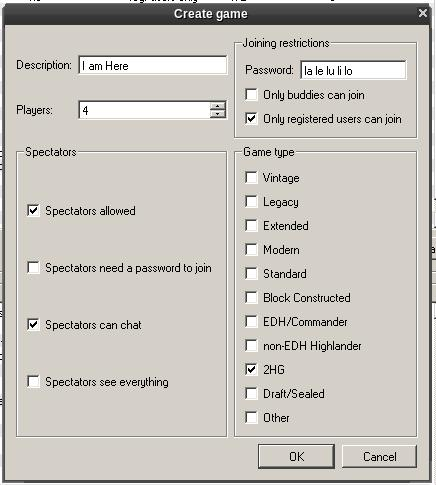
\includegraphics[scale=0.5]{pics/fetch54df}
\end{center}

Here are all of the options for creating a game:
\begin{description}
 \item[Description] Describe the game in your own words (i.e. “Competitive Standard”, “Casual EDH- No Infinites”, “RavnicaDraft”, “Here is Chris”)
 \item[Players] Specify the number of Players in the game. This cannot be changed after the game is created. The game can only begin when the specified number of players join.
 \item[Spectators] Spectators are users that are in a game, but they are not one of the players. Spectators can see all of the public zones of the game and everything displayed in the Info/Chat Bar. Any number of users can join a game as a Spectator (as long as the “Spectators Allowed” box is checked).
 \begin{description}
  \item[Spectators Allowed] Unchecking this box will prohibit any/all users from joining the game as a Spectator.
  \item[Spectators Need a Password to Join] Checking this box will make it so that in order for a user to join as a Spectator, they need to type the password you specify in the Password Field.
  \item[Spectators can Chat] Checking this box will allow Spectators to type comments in the Chat bar during the game.
  \item[Spectators See Everything] Checking this box will allow Spectators to view cards in all private zones of all players (hands, libraries, face-down cards).
 \end{description}
 \item[Password Field] If you type anything in this field, a Player (or Spectator if the “Spectators Need Password” box is checked) will need to type the exact same thing you typed in order to join the game (and it is case-sensitive).
 \item[Only Buddies Can Join] Checking this box will prevent any user who is not in your Buddy List from joining the game as a Player or Spectator. NOTE: Your username is not on your buddy list. If you leave a game you created, and this box is checked, you will not be able to rejoin.
 \item[Only Registered Users Can Join] Checking this box will prevent anyone who has not registered on the Cockatrice website from joining as a Player or Spectator.
 \item[Game Type] These check boxes have no effect on the game. They inform other Users browsing the Games list of what format your game is. Users can choose to view only games of a certain Type/Format. (\url{http://en.wikipedia.org/wiki/Magic:_The_Gathering_formats})
\end{description}

\subsection{Joining a Game}
Most of the time, to join a game you click on the “MTG Room” tab, click on a game in the Games list, then click Join. If the Game's creator specified a password then you will have to type that password in a small window that appears after you click Join (the password is case-sensitive). If your User Profile meets the criteria of the Game's creator then a new tab will open with that game. There is also an easy way to join a game in which a User in your Buddy List is playing. Go to the “User Lists” tab, right click any Username from the Buddies Online list (at the left of the window) to make a menu appear, and select “Show this user's games”. A window will open with a list of games that the User is either playing or watching. In the same manner as described with the “MTG Room” tab, simply click on a game and click Join. To watch a game, the instructions are the same except that you click the “Join as Spectator” button instead of the Join button. NOTE: If you are a player in a game and you wish to become a spectator in that game, you must first leave the game then rejoin as a Spectator. Same thing if you are a Spectator and wish to play.

\subsection{Searching for Games}
The Games list in the “MTG Room” tab displays by default all games that have not reached the specified number of players. The “Filter Games” button makes looking through this list easier if you are looking to join a particular kind of game. When this button is selected, a window appears (see below).
\begin{center}
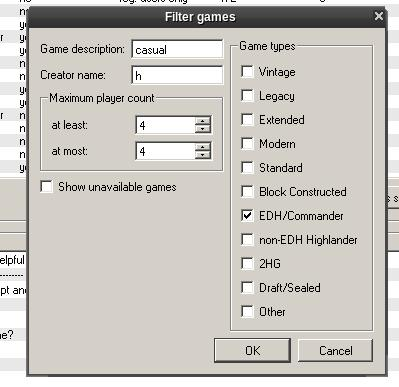
\includegraphics[scale=0.5]{pics/fetchd30e}
\end{center}
\begin{description}
 \item[Game Description] Displays games with certain descriptions. You can even search partial names.
 \item[Creator] Displays games created by Users with that username. It even searches for partial names.
 \item[Player Count] Displays all games where the specified number of players is greater-than or equal to the “at least” number and less-than or equal to the “at most” number. For instance, setting both numbers to 3 will display all games whose creators made as 3-player games.
 \item[Show Unavailable Games] Checking this box will display games that are full and in progress. You can still join these games as a Spectator if the game's creator allows it.
 \item[Game Types] Displays games with the selected types. Bear in mind that the Cockatrice software does not enforce deck construction for formats. So just because a game's type is EDH/Commander, doesn't necessarily mean that is what's being played in the game. Players can agree to switch formats in a game.
\end{description}

\section{Keeping Track of Buddies}


Cockatrice allows registered users to keep track of other registered users in a buddy list. You won't be able to do anything with this list (or other registered users at all) unless you are a registered user and connected to the server.

To add a User to your Buddy list, right-click their username and, in the menu that appears, select “Add to buddy list”. You can right-click and add a User in this manner anywhere you see their username (under the “User lists” tab, the “MTG Room” tab, in a game, or in a direct chat). When you add a User, their username will appear in the list “Buddies Online” located under the “User lists” tab. If the username appears in a light shade of gray, then that User is not connected to the server. If it appears in black, then that User is connected to the server.

If you see that one of your Buddies is connected, you can see the games he/she is currently in. Right-click their username, and in the menu that appears select “Show this user's games”. A window will appear from which you can watch or play in a game that your buddy is currently in.

You can Direct Chat with a Buddy (or any user for that matter) by right-clicking their username and, from the menu that appears, selecting “Direct Chat”. When you do this, a new tab will open (both on your window and on the other User's window) containing a chat room that can only be seen and used by the two of you. The place where you type in your messages is at the very bottom of the window.

To remove a User from your Buddy list, right-click their username, and from the menu that appears select “Remove from buddy list”.

\section{Dealing with and Preventing Unpleasantries}
Make a screenshot, there are several free programs available.
Right-Click a username to add to Ignore List.

\chapter{Frequently Asked Questions (FAQ)}
\section{How to update the card database}
\section{Change Card Art / Custom Card Art}
\section{Use Higher Resolution Cards}
\section{Booster drafts}
\section{What is Legacy / Vintage / EDH?}
\section{Linking cards and URLs in the Cockatrice chat.}



\listoffigures
\listoftables
\printindex

\end{document}